%----------------------------------------------------------------------------------------------
%--------------------------     5 Eigenwerte / Eigenvektoren    -------------------------------
%----------------------------------------------------------------------------------------------
\section{Eigenwerte / Eigenvektoren}   

Ein Vektor $\vec{v}$ heisst Eigenvektor der $n \times n$ Matrix $A$ zum Eigenwert $\lambda$, wenn 
$$A \vec{v} = \lambda \vec{v} \quad \text{und} \quad \vec{v \neq 0}$$


\subsubsection{Eigenschaften}

\begin{itemize}
	\item Ein Eigenvektor $\vec{v}$ wird durch die Matrix $A$ nur gestreckt (Streckungsfaktor $\lambda$)
	\item Es gibt maximal $n$ verschiedene Eigenwerte $\lambda$
	\item Zu jedem Eigenwert gibt es unendlich viele Eigenvektoren
\end{itemize}


%----------------------------------------------------------------------------------------------
%----------------------     5.1 Eigenwerte und Eigenvektoren finden    ------------------------
%----------------------------------------------------------------------------------------------
\subsubsection{Eigenwerte und Eigenvektoren finden}
	
\begin{enumerate}
	\item Eigenwertproblem: $A \crd{\vec{v}} = \crd{\lambda \vec{v}}$ \textrightarrow\  $(A - \lambda E) \vec{v} = 0$
	\item Charakteristische Gleichung: $\det(A -  \crd{\lambda} I) = 0$
	\item Berechnung der Eigenwerte \crd{$\lambda_i$} als Lösungen der charakteristischen Gleichung
	\item Berechnung der Eigenvektoren \crd{$\vec{v}_i$} mittels Gauss-Algorithmus: $(A - \lambda_i I) \vec{v}_i = 0$
	\item Resultat kontrollieren: $A \vec{v}_i = \lambda_i \vec{v}_i$
\end{enumerate}


\example{Eigenwerte und Eigenvektoren berechnen}

\begin{center}
	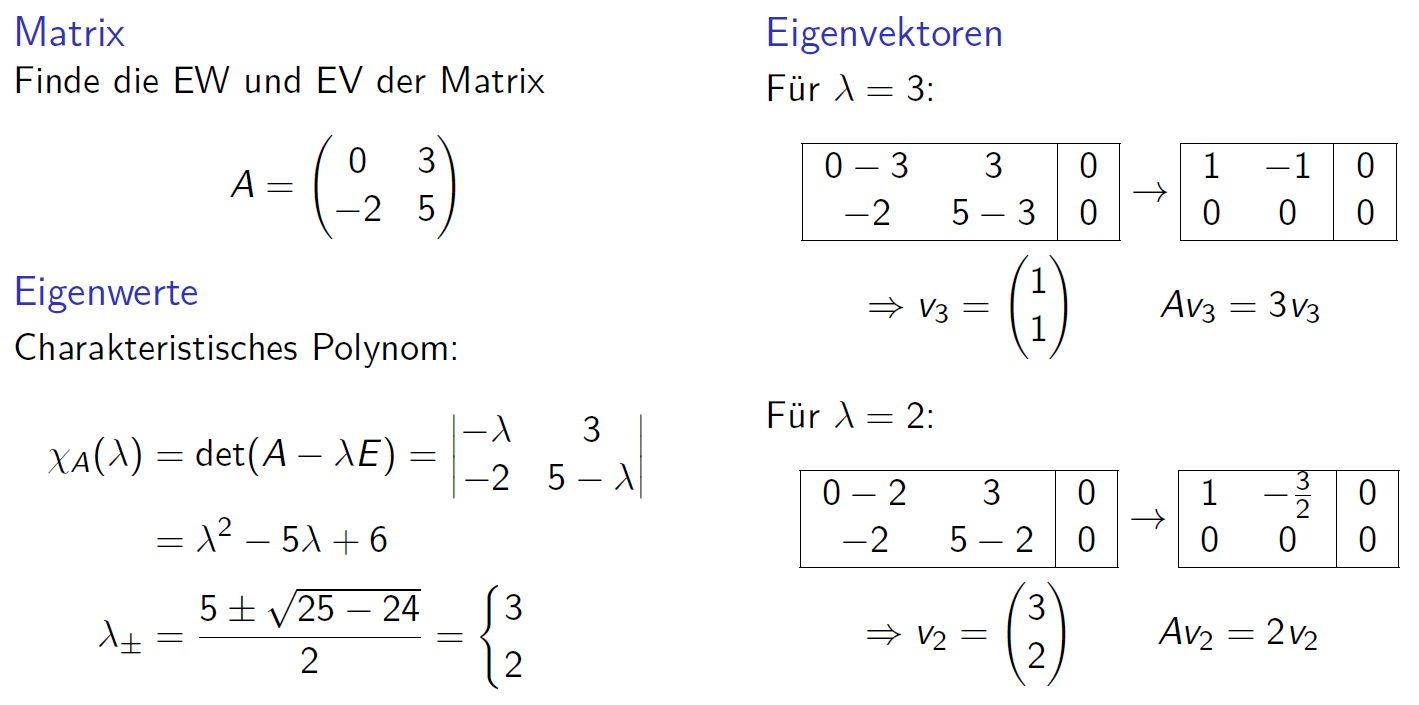
\includegraphics[width=0.85\linewidth]{images/eigenwerte-eigenvektoren.PNG} 
\end{center}


\subsubsection{Spezialfall -- Eigenwerte und Eigenvektoren}

Wenn $A A^t$ oder $A^t A$ eine Zeile und Spalte mit nur
einem Zahleneintrag enthalten, so ist die Zahl ein Eigenwert zum zugehörigen Standardbasisvektor. \\
Die weiteren EW und EV können ohne diese Zeile / Spalte berechnet werden!	   


\example{Spezialfall}

\begin{minipage}{0.35\linewidth}
	$$ AA^t = \begin{pmatrix} 2 & 0 & -2 \\ 0 & 9 & 0 \\ -2 & 0 & 2 \end{pmatrix} $$
	$$ A_0 = \begin{pmatrix}2 & -2 \\ -2 & 2 \end{pmatrix} $$						
\end{minipage}	
\hfill
\begin{minipage}{0.55\linewidth}
	\begin{center}
		Aus $AA^t$ kann man $\lambda = 9$ direkt ablesen.
		$$ \text{Daraus folgt: }\vec{v}_{\lambda} = \begin{pmatrix} 0 \\ 1 \\ 0 \end{pmatrix} $$
	\end{center}
\end{minipage}		


%----------------------------------------------------------------------------------------------
%---------------------------     5.2 Eigenschaften der Matrix    ------------------------------
%----------------------------------------------------------------------------------------------
\subsection[Eigenschaften der Matrix A bzgl. Eigenwerte]{Eigenschaften der Matrix $A$ bzgl. Eigenwerte}

\begin{itemize}
	\item $\operatorname{spur}(A) = \operatorname{spur}(A') =$ Summe der Eigenwerte von $A$ 
	\item $\det(A) = \det(A') =$ Produkt aller Eigenwerte von $A$
\end{itemize}


\subsubsection{Rechenregeln Eigenwerte}

\vspace{-0.2cm}
$$ \frac{1}{\lambda} = \lambda - 1 $$	
			   

%----------------------------------------------------------------------------------------------
%-------------------------     5.3 Diagonalisierung einer Matrix    ---------------------------
%----------------------------------------------------------------------------------------------
\subsection{Diagonalisierung einer Matrix}
		
Mit Diagonalmatritzen kann man einfach rechnen.

\textbf{Eine Matrix ist diagonalisierbar, wenn:} 
\vspace{0.1cm}
\begin{itemize}
	\item Die Matrix symmetrisch ist , also $A = A^t$
	\item \textbf{Eine Basis aus Eigenvektoren existiert}
\end{itemize}
			
		
\subsubsection{Vorgehen Matrix diagonalisieren} 

\begin{enumerate}
	\item Eigenbasis $C$ aus $n$ linear unabh. Eigenvektoren finden \\
		\textrightarrow\ Spalten von $C$ sind Eigenvektoren
	\item Basis-Transformationsmatrix $T$ berechnen: $T = C^{-1}$ \\
		\textrightarrow\ Matrix aus Eigenvektoren invertieren
	\item Diagonalisierte Matrix $A'$ berechnen: $A' = T A T^{-1}$ \\
		\textrightarrow\ $A'$ enhält Eigenwerte auf Diagonalen
\end{enumerate}

\vspace{0.2cm}

\begin{center}
	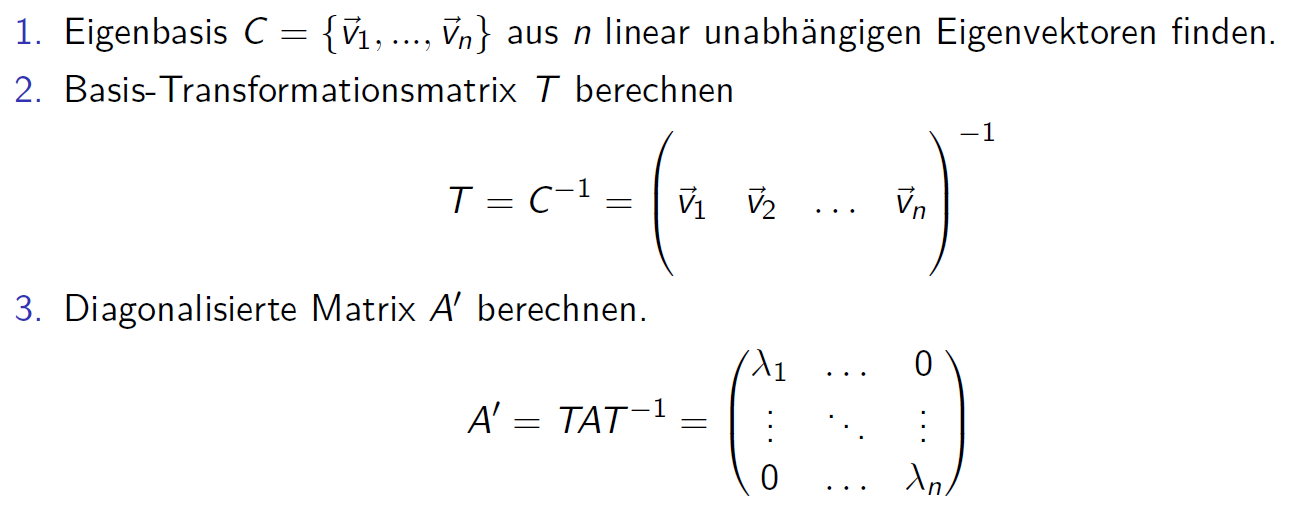
\includegraphics[width=0.7\linewidth]{images/matrix-diagonalisieren.PNG} 
\end{center}

\subsubsection{Transformationsmatrix $T$ und Eigenbasis $C$}

\begin{itemize}
	\item Die Eigenbasisis-Matrix $C$ enthält in ihren Spalten die Eigenvektoren der Matrix $A$ (Anfangsmatrix) 
	\item Die Transformationsmatrix $T$ ist die Inverse von $C$
\end{itemize}

		
\subsubsection{Spezialfall Symmetrische Matrix diagonalisieren}
		
Die Eigenvektoren einer symmetischen Matrix sind orthagonal 
		

%----------------------------------------------------------------------------------------------
%---------------------------     5.4 Singulärwertzerlegung (SVD)    ---------------------------
%----------------------------------------------------------------------------------------------
\subsection{Singulärwertzerlegung (SVD)}

Eine $m \times n$ Matrix $A$ wird zerlegt in zwei orthagonale Matritzen und eine Diagonalmatrix
$$ A = U \, \Sigma \, V^t$$	 

\begin{tabular}{ll}
	$U$ 		& Orthagonale $m \times m$ Matrix  ($U$ diagonalisiert $A A^t$)		\\
	$V$ 		& Orthagonale $n \times n$ Matrix ($V$ diagonalisiert $A^t A$)		\\
	$V^t$ 		& Transponierte von $U$ 											\\
	$\Sigma$ 	& Diagnonalmatrix mit $r$ Singulärwerten $\sigma_0$ bis $\sigma_r$
\end{tabular}			 

\begin{center}
	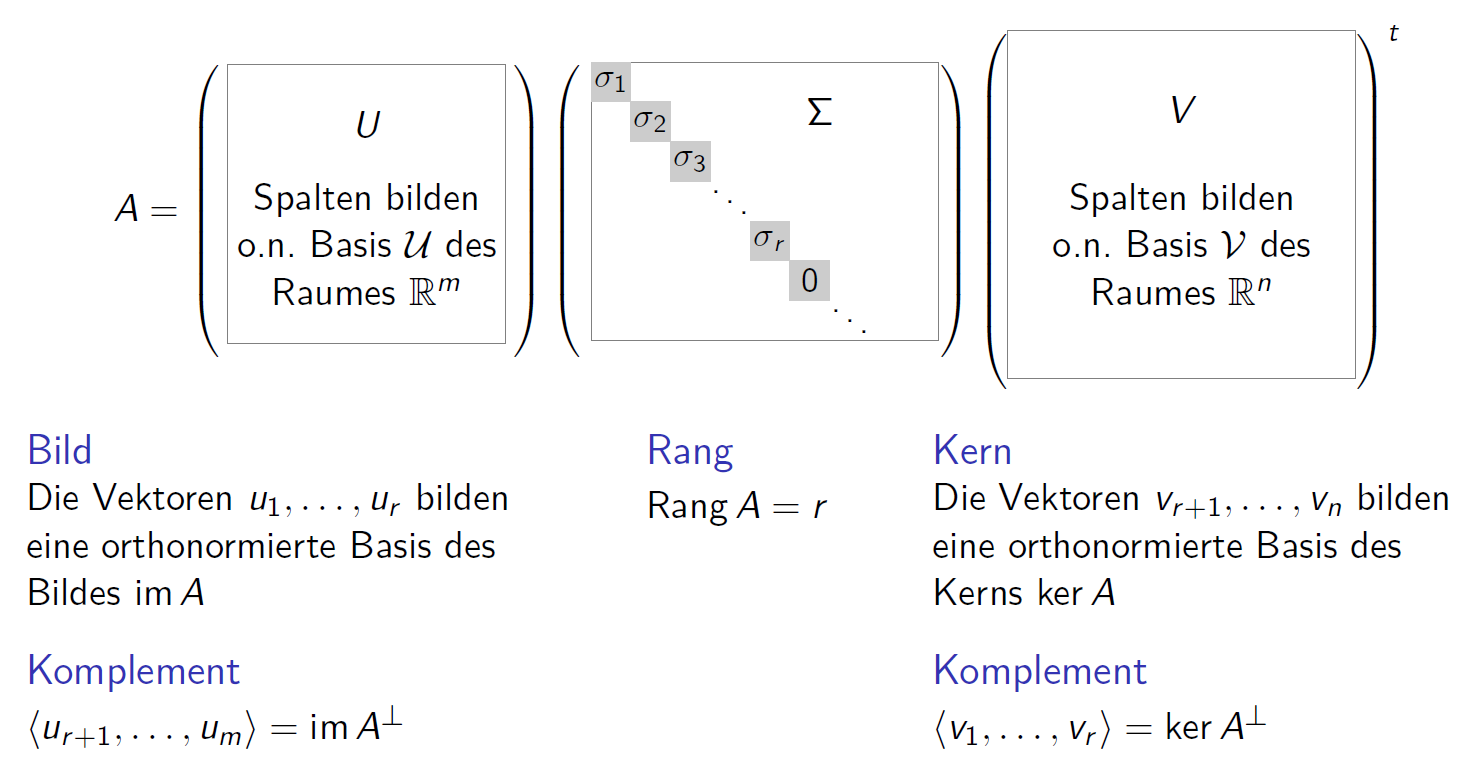
\includegraphics[width=0.7\linewidth]{images/SVD.PNG}
\end{center}
	

\subsubsection{Vorgehen Singulärwertzerlegung}

\begin{enumerate}
	\item $A A^t$ und $A^t A$ berechnen
	\item Eigenwerte von $A A^t$ oder $A^t A$ berechnen (EW identisch)
	\item Eigenwerte der Grösse nach sortieren: $\sigma_1 \geq \sigma_2 \geq \ldots \geq \sigma_r \geq 0$
	\item $V =$ auf Länge 1 normierte Eigenvektoren von $A^t A$
	\item $U =$ Spalten $u_i$ mit $u_i = \frac{A v_i}{\vert A v_i \vert}$
	\item Singulärwerte bestimmen: $\sigma_i = \sqrt{\lambda_i}$ und Matrix $\Sigma$ füllen
	\item Kontrolle mit $A = U \, \Sigma \, V^t$
\end{enumerate}


%----------------------------------------------------------------------------------------------
%-----------------------------------     5.4 Pseudoinverse    ---------------------------------
%----------------------------------------------------------------------------------------------		
\subsection{Pseudoinverse}

\textbf{Die Pseudoinverse löst  Gleichungssysteme mit der Lösung minimaler Länge}

\textrightarrow\ $\abs{\vec{x}}$ ist minimal
		
\begin{center}
	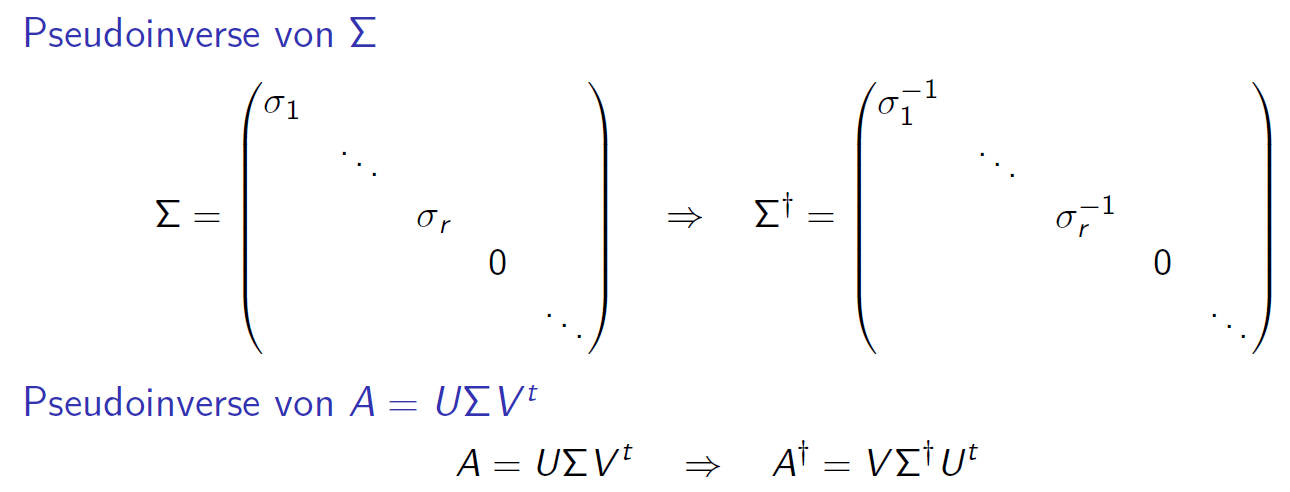
\includegraphics[width=0.8\linewidth]{images/pseudoinverse.PNG}
	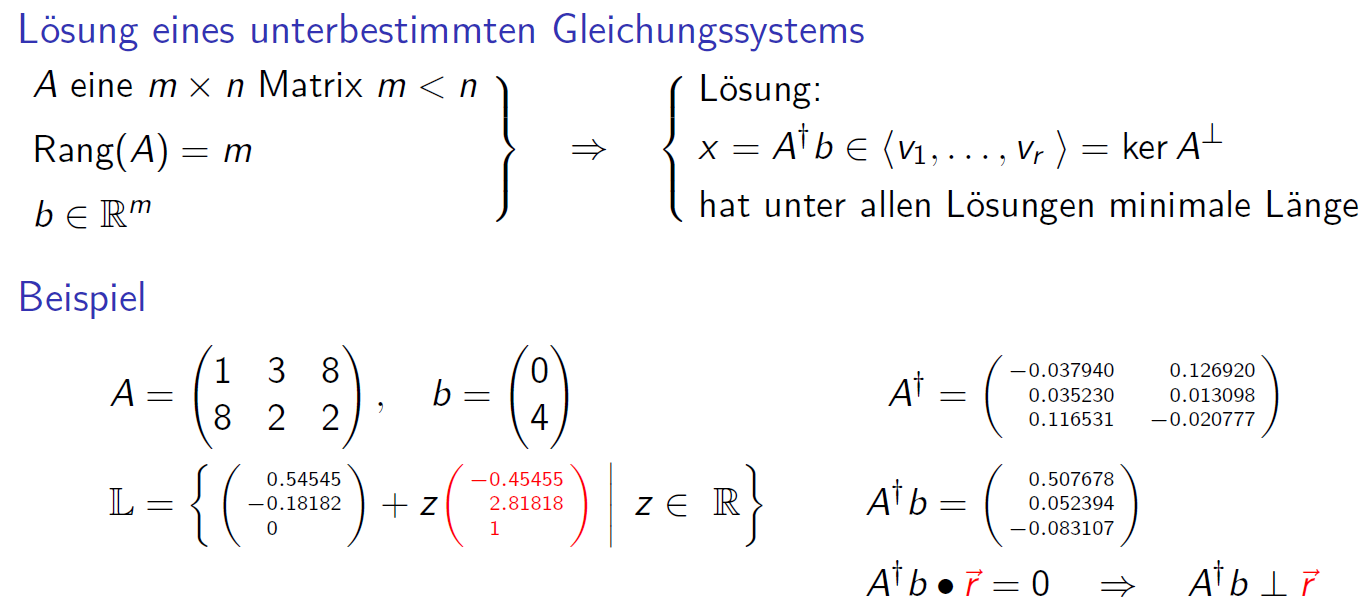
\includegraphics[width=0.8\linewidth]{images/pseudoinverse2.PNG}
\end{center}

			